%\documentclass[12pt, twoside]{book}
\documentclass[12pt, oneside]{book}  % jednostranna tlac
\usepackage[a4paper,top=2.5cm,bottom=2.5cm,left=3.5cm,right=2cm]{geometry}
\usepackage[utf8]{inputenc}
\usepackage[T1]{fontenc}
\usepackage{graphicx}
\usepackage{url}
\usepackage{subfig}
\usepackage{amsmath}
\usepackage{amsthm}
\usepackage{amssymb}
\usepackage{multirow}
\usepackage{textcomp}
\usepackage[table,xcdraw]{xcolor}
\usepackage[hidelinks,breaklinks]{hyperref}


%\usepackage[slovak]{babel} % vypnite pre prace v anglictine
\linespread{1.25} % hodnota 1.25 by mala zodpovedat 1.5 riadkovaniu

% -------------------
% --- Definicia zakladnych pojmov
% --- Vyplnte podla vasho zadania
% -------------------
\def\mfrok{2020}
\def\mfnazov{Efficient Convolutional Neural Networks Recognizing Driveable Trails}
\def\mftyp{Master's Thesis}
\def\mfautor{Bc. Adrián Matejov}
\def\mfskolitel{Mgr. Pavel Petrovič, PhD.}
\def\mfkonzultant{Mgr. Marek Šuppa}  

\def\mfmiesto{Bratislava, \mfrok}
\def\mfodbor{Computer Science}
\def\program{Computer Science}
\def\mfpracovisko{Department of Applied Informatics}

\begin{document}
\frontmatter


% -------------------
% --- Obalka ------
% -------------------
\thispagestyle{empty}

\begin{center}
\sc\large
Comenius University in Bratislava\\
Faculty of Mathematics, Physics and Informatics

\vfill

{\LARGE\mfnazov}\\
\mftyp
\end{center}

\vfill

{\sc\large 
\noindent \mfrok\\
\mfautor
}

\cleardoublepage
% --- koniec obalky ----

% -------------------
% --- Titulný list
% -------------------

\thispagestyle{empty}
\noindent

\begin{center}
\sc  
\large
Comenius University in Bratislava\\
Faculty of Mathematics, Physics and Informatics

\vfill

{\LARGE\mfnazov}\\
\mftyp
\end{center}

\vfill

\noindent
\begin{tabular}{ll}
Study Programme: & \program \\
Field of Study: & \mfodbor \\
Department: & \mfpracovisko \\
Supervisor: & \mfskolitel \\
Consultant: & \mfkonzultant \\
\end{tabular}

\vfill


\noindent \mfmiesto\\
\mfautor

\cleardoublepage
% --- Koniec titulnej strany


% -------------------
% --- Zadanie z AIS
% -------------------
% v tlačenej verzii s podpismi zainteresovaných osôb.
% v elektronickej verzii sa zverejňuje zadanie bez podpisov
% v pracach v naglictine anglicke aj slovenske zadanie

\newpage 
\thispagestyle{empty}
\hspace{-2cm}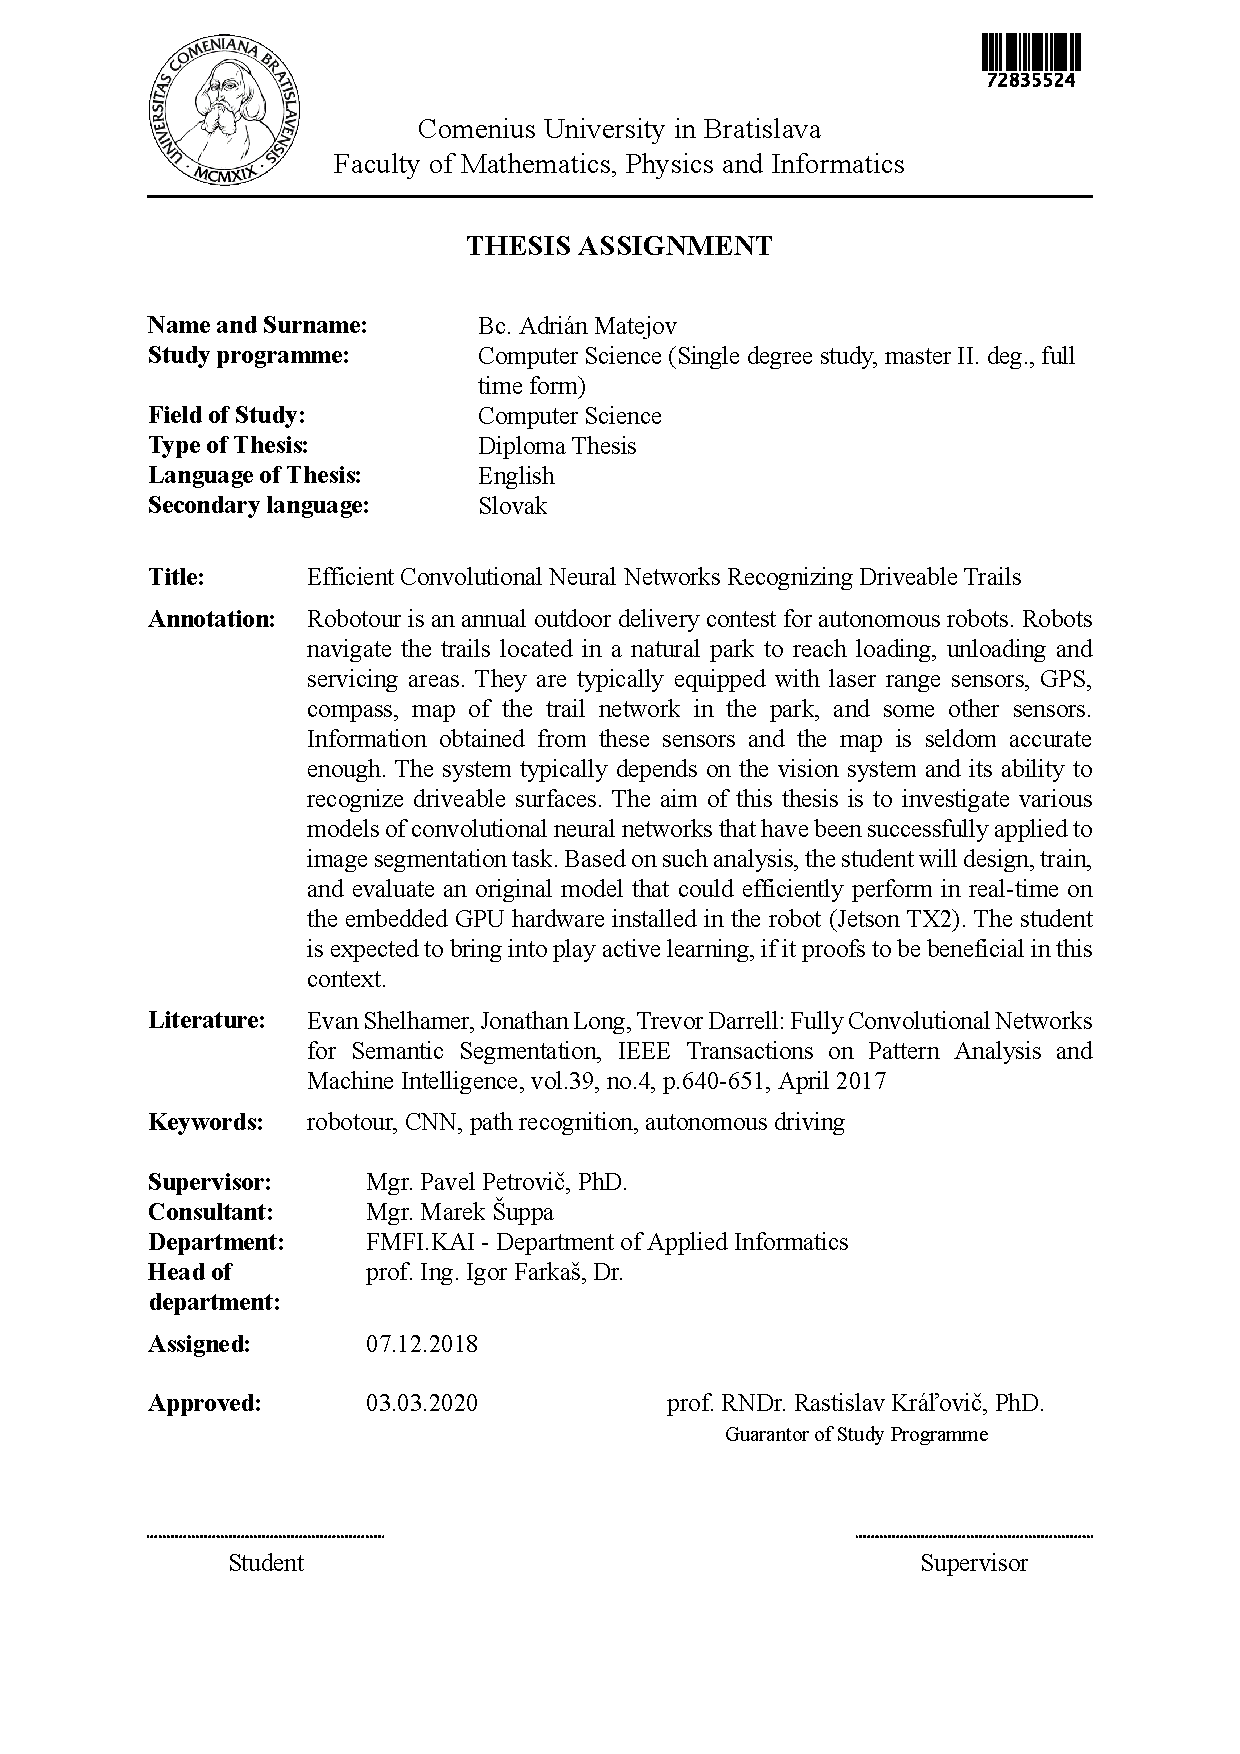
\includegraphics[width=1.1\textwidth]{assignments/zadanie_english}
\newpage 
\thispagestyle{empty}
\hspace{-2cm}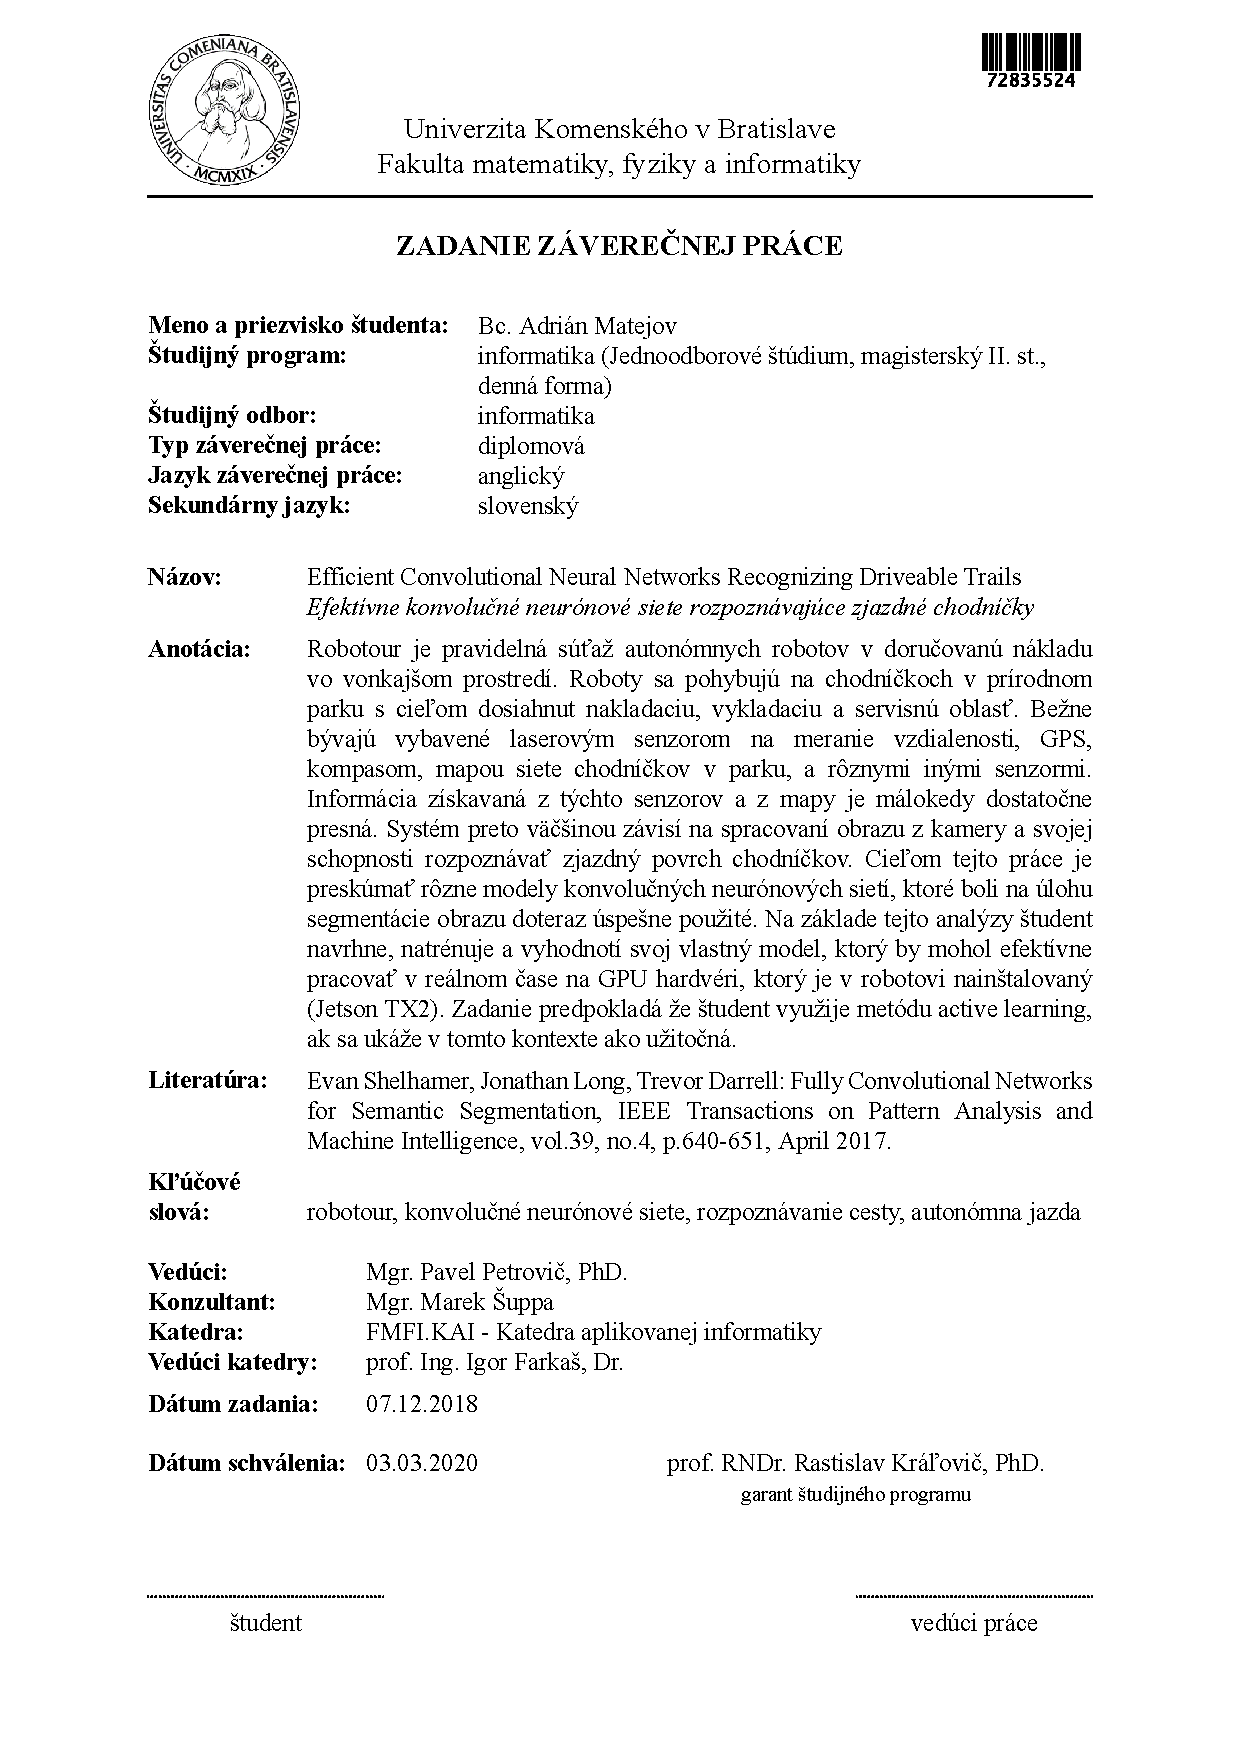
\includegraphics[width=1.1\textwidth]{assignments/zadanie_slovak}

% --- Koniec zadania

\frontmatter

% -------------------
%   Poďakovanie - nepovinné
% -------------------
\setcounter{page}{3}
\newpage 
~

\vfill
{\bf Acknowledgement:} I would like to thank my supervisor Mgr. Pavel
Petrovič, PhD. for leading this thesis, capturing images and labeling both datasets,
reviewing this thesis and for the opportunity to participate at the RoboTour contests.
A tremendous thanks goes to my both friend and consultant Mgr. Marek Šuppa
for helpful advises, consultations, new ideas, thorough thesis review
and last but not least, for providing me with his own GPU machine in order to
conduct the experiments.
Special thanks goes to my closest ones for their continuous support throughout my studies.

% --- Koniec poďakovania

% -------------------
% --- Abstrakt - Anglicky 
% -------------------
\newpage 
\section*{Abstract}

Our faculty's students annually participate at the competition called RoboTour
Outdoor Delivery Contest. The robot, which the faculty has at its disposal, had
been designed, built and improved in previous works.
One of the rules of this competition strictly forbids the robot from leaving driveable trail.
Since the previous approaches have not
been accurate enough, we focus on solving the problem of recognizing driveable trails
using deep learning, whose application to various areas has achieved remarkable success
in recent years.
In this work we firstly deal with this problem by utilizing existing convolutional
neural network models for semantic segmentation and test them right at the competition
in the outdoor environment. These models reach very good results and the robot is
able to distinguish between driveable and non-driveable segments more accurately,
which contributes to a better navigation.
In order to reach higher prediction speed, we minimize the size of these models
and reach more than double speedup with prediction of the road. Subsequently, we
compare our models with the ones specifically designed for devices with lower
computational power.
Finally, we examine the possibilities of reducing the number of images needed for
training, leading to less effort dedicated to labeling. Our simulations
show that by making use of image clustering combined with entropy of prediction
it is possible to halve the number of training data at the cost of a very little
decrease in accuracy.

\paragraph*{Keywords:} robotour, CNN, path recognition, autonomous driving

% --- Koniec Abstrakt - Anglicky

% -------------------
%   Abstrakt - Slovensky
% -------------------
\newpage 
\section*{Abstrakt}

Študenti našej fakulty sa každoročne zúčastňujú súťaže RoboTour Outdoor Delivery Contest.
Robot, ktorého má fakulta k dispozícii, bol navrhnutý, skonštruovaný a
vylepšovaný v predošlých prácach. Jedno z pravidiel tejto súťaže prísne zakazuje
robotovi opustiť chodníček.
Keďže predošlé prístupy neboli dostatočne presné, v tejto práci riešime
problém rozpoznávania zjazdných chodníčkov z obrázka pomocou hlbokého učenia,
ktorého aplikácia v rôznych oblastiach dosahuje pozoruhodné výsledky.
Najskôr využívame už existujúce modely konvolučných neurónových sietí na sémantickú
segmentáciu, ktoré testujeme priamo na súťaži vo vonkajšom prostredí. Tieto modely
dosahujú veľmi dobré výsledky a robot vie oveľa presnejšie rozlišovať medzi zjazdnými
a nezjazdnými segmentami, čo prispieva k lepšej navigácii.
Aby sme dosiahli vyššiu rýchlosť predpovedania, zmenšujeme veľkosti týchto modelov,
čím dosahujeme viac ako dvojnásobné zrýchlenie pri predpovedaní cesty. Následne naše
modely porovnávame s takými, ktoré boli navrhované priamo na zariadenia s nižším výpočtovým
výkonom.
Nakoniec skúmame možnosti zníženia počtu obrázkov potrebných pri trénovaní,
čo vedie k zníženiu času stráveného označovaním obrázkov.
Naše simulácie ukazujú, že využitím zoskupovania podobných obrázkov
v kombinácii s entropiou predpovedí vieme zredukovať počet trénovacích dát na polovicu
za cenu veľmi malého zníženia v presnosti.

\paragraph*{Kľúčové slová:} robotour, konvolučné neurónové siete, rozpoznávanie cesty, autonómna jazda
% --- Koniec Abstrakt - Slovensky


% -------------------
% --- Obsah
% -------------------

\newpage 

\tableofcontents

% ---  Koniec Obsahu

% -------------------
% --- Zoznamy tabuliek, obrázkov - nepovinne
% -------------------

\newpage 

\listoffigures
\listoftables

% ---  Koniec Zoznamov

\mainmatter


\input introduction.tex 

\input 01_preliminaries.tex

\input 02_relatedWork.tex

\input 03_testingandcomparing.tex

\input 04_smallermodels.tex

\input 05_activelearning.tex

\input conclusion.tex

% -------------------
% --- Bibliografia
% -------------------


\newpage	

\backmatter

\thispagestyle{empty}
\nocite{*}
\clearpage

\bibliographystyle{unsrt}
\bibliography{literature}

%---koniec Referencii

% -------------------
%--- Prilohy---
% -------------------

%Nepovinná časť prílohy obsahuje materiály, ktoré neboli zaradené priamo  do textu. Každá príloha sa začína na novej strane.
%Zoznam príloh je súčasťou obsahu.
%
\input appendix_a.tex
\addcontentsline{toc}{chapter}{Appendix A}

%
%\addcontentsline{toc}{chapter}{Appendix B}
%\input AppendixB.tex

\end{document}
